\documentclass[12pt,letterpaper,titlepage]{article}

\usepackage{fontspec}
\defaultfontfeatures{Mapping=tex-text}
\usepackage{xunicode}
\usepackage{xltxtra}
\usepackage{amsmath}
\usepackage{pdfpages}
\usepackage{amsfonts}
\usepackage{bbold}
\usepackage{amssymb}
\setcounter{secnumdepth}{0}
\usepackage{nameref}
\usepackage{enumitem}
\usepackage{environ}
\usepackage{pgfplots}
\usepackage{listings}

\showboxdepth=\maxdimen
\showboxbreadth=\maxdimen


\usepackage{paracol}
\usepackage{wrapfig}
\globalcounter{table}
\globalcounter{figure}
\usepackage{graphicx}
\usepackage[left=1in,right=1in,top=1in,bottom=1in]{geometry}
\graphicspath{{img/}}

\author{Jacob Abel}
\title{	Design \& Simulate 14
	\\\large ECE2204 CRN:82929
}

\setlength{\parskip}{0.5em}

\begin{document}
\maketitle
\begin{raggedright}

\section{Problem 14.10-8.a.1: } Switched from NMOS to PMOS.
\subsection{Design}

Design a MOSFET current source circuit to meet the following specifications. The circuit to be designed has the configuration shown below with all NMOS transistors swapped with PMOS transistors and $V^+$ swaps places with $V^-$.  The bias voltages are $V^+ = 2.5V$ and $V^-=0$. Transistors are available with parameters $k_p^\prime = 100\mu A/V^2$, $V_{TP} = 0.4V$. and $\lambda = 0$. Design the circuit such that $I_{REF} = 100\mu A$, $I_O = 60\mu A$, and $V_{SD2}(sat) = 0.4V$.

\begin{center}
\begin{paracol}{2}
\centering
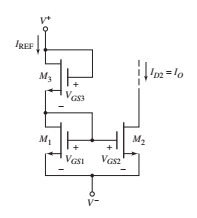
\includegraphics[width=\textwidth, height=12\baselineskip, keepaspectratio=true]{ds1}

(Original)
\switchcolumn
\centering
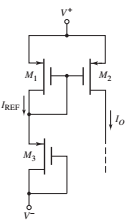
\includegraphics[width=\textwidth, height=12\baselineskip, keepaspectratio=true]{ds1a}

(w/ PMOS and Voltage Inversion)
\end{paracol}
\end{center}

\begin{align*}
\\ V_{SD2}(sat) 
	&= V_{SG2} + V_{TP}
\\ V_{SG2}
	&= V_{SG1}
	 = V_{SD2}(sat) - V_{TP}
	 = 0.4V + 0.4V
	 = 0.8V
\\ \frac{W}{L}_2 
	&= \frac{2I_O}{k_p^\prime(V_{SG2}+V_{TP})^2}
	 = \frac{2(60\mu A)}{(100\mu A/V^2)(0.8V-0.4V)^2}
	 = 7.5
\\ \frac{W}{L}_1 
	&= \frac{2I_{REF}}{k_p^\prime(V_{SG1}+V_{TP})^2}
	 = \frac{2(100\mu A)}{(100\mu A/V^2)(0.8V-0.4V)^2}
	 = 12
\\ V_{SG3}
	&= V^+ - V^- - V_{GS1}
	 = 2.5V - 0V - 0.8V
	 = 1.7V
\\ \frac{W}{L}_3 
	&= \frac{2I_{REF}}{k_p^\prime(V_{SG3}+V_{TP})^2}
	 = \frac{2(100\mu A)}{(100\mu A/V^2)(1.7V-0.4V)^2}
	 = 1.183
\end{align*}

The final design values are $\frac{W}{L}_1 = 12$, $\frac{W}{L}_2 = 7.5$, and $\frac{W}{L}_3 = 1.183$.

\clearpage
\subsection{Validation}

\begin{center}
LTSpice Implementation (values within $<1\%$)
\columnratio{0.5}
\begin{paracol}{2}
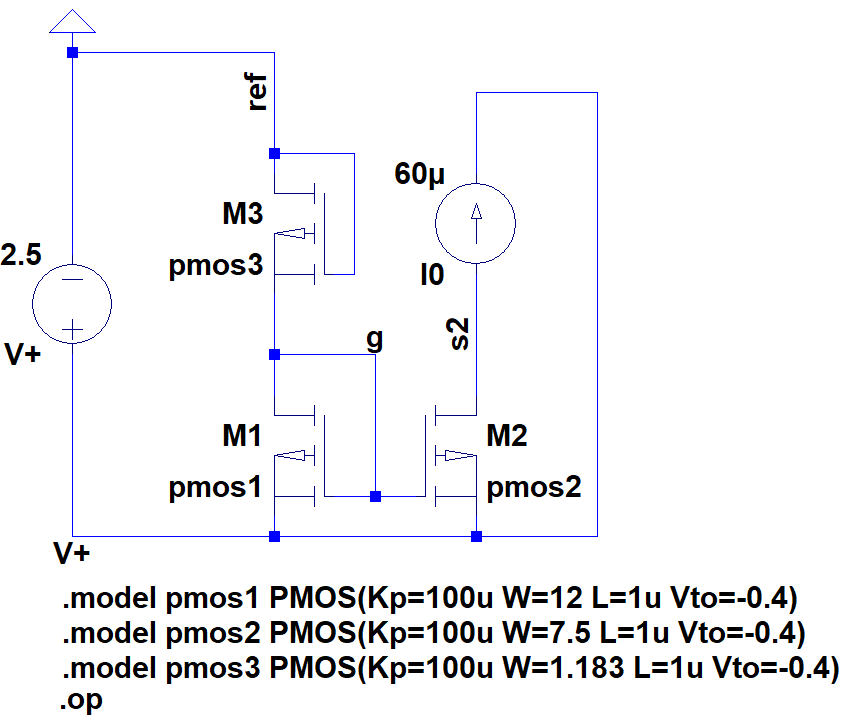
\includegraphics[width=.48\textwidth, height=\textheight, keepaspectratio=true]{ds1b}
\switchcolumn
\begin{tabular}{|l|l|c|}
  \hline V(g):	   & 1.69378	   & voltage
\\\hline V(v+):	   & 2.5	       & voltage
\\\hline V(s2):	   & 2.5	       & voltage
\\\hline Id(M2):   & -5.99248e-005 & device\_current
\\\hline Ig(M2):   & -0	           & device\_current
\\\hline Ib(M2):   & 2.72735e-019  & device\_current
\\\hline Is(M2):   & 5.99248e-005  & device\_current
\\\hline Id(M1):   & -99.0091	   & device\_current
\\\hline Ig(M1):   & -0	           & device\_current
\\\hline Ib(M1):   & 8.16221e-013  & device\_current
\\\hline Is(M1):   & 99.0091	   & device\_current
\\\hline Id(M3):   & -99.0091	   & device\_current
\\\hline Ig(M3):   & -0	           & device\_current
\\\hline Ib(M3):   & 1.70378e-012  & device\_current
\\\hline Is(M3):   & 99.0091	   & device\_current
\\\hline I(I0):	   & 6e-005	       & device\_current
\\\hline I(V+):	   & -99.0091	   & device\_current
\\\hline
\end{tabular}
\end{paracol}
\begin{align*}
   Err_{V_{SG1}} &= \frac{|1.7-1.69378|}{1.7} = 0.0037 = 0.37\%
\\ Err_{I_{REF}} &= \frac{|100-99.0091|}{100} = 0.0099 = 0.99\%
\\ Err_{I_O} &= \frac{|60-59.9248|}{60} = 0.00125 = 0.13\%
\end{align*}
\end{center}

\clearpage
\section{Problem 14.10-8.b.1: } Derived from Problem 10.54 from page 744 of the textbook by changing some values and adding a 5th transistor.

\columnratio{0.75}
\begin{paracol}{2}
\switchcolumn*
\begin{center}
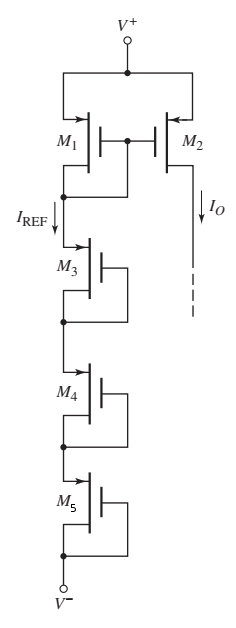
\includegraphics[width=\textwidth, height=20\baselineskip, keepaspectratio=true]{ds2}
\end{center}
\switchcolumn
\subsection{Design}
The transistor circuit shown to the left is biased at $V^+ = 12V$ and $V^- = 0V$. The transistor parameters are $V_{TP} = -1.2V$, $k_p^\prime = 80\mu A/V^2$, $\lambda = 0$, $\frac{W}{L}_1 = \frac{W}{L}_2 = 25$, and $\frac{W}{L}_3 = \frac{W}{L}_4 = \frac{W}{L}_5 = 4$. Determine $I_{REF}$, $I_O$, and $V_{SD2}(sat)$.

$V_{SG1} = V_{SG2}$, $V_{GD1} = V_{GD2} = V_{GD3} = V_{GD4} = V_{GD5} = 0V$

\begin{align*}
   V^+ &= {SG1} + V_{SG3} + V_{SG4} + V_{SG5} 
\\\implies& V_{SG3} + V_{SG4} + V_{SG5} = 3V_{SG3}
\\\implies& V_{SG1} = V^+ - 3V_{SG3}
\end{align*}

Ran out of time and was unable to complete the second problem. 

%The reference current is $I_{REF} = $, the output current is $I_O = $, and transistor two's saturation voltage is $V_{SD2}(sat) = $.

\end{paracol}
%\clearpage
%\subsection{Validation}
%
%\begin{center}
%LTSpice Implementation (values within $<1\%$)
%\columnratio{0.5}
%\begin{paracol}{2}
%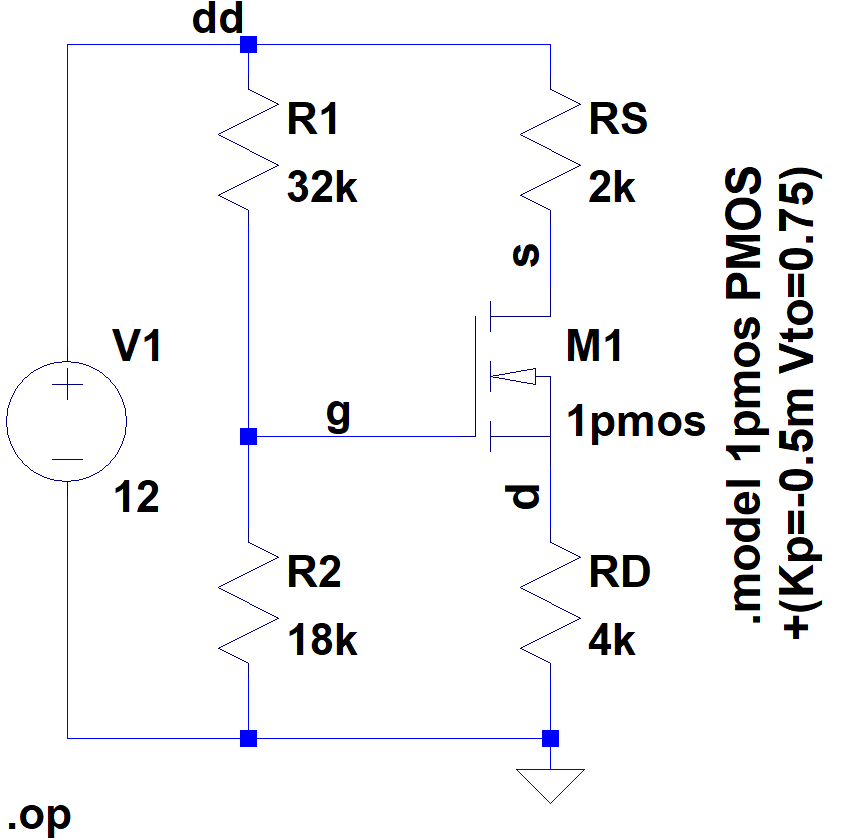
\includegraphics[width=.47\textwidth, height=\textheight, keepaspectratio=true]{ds2b}
%\switchcolumn
%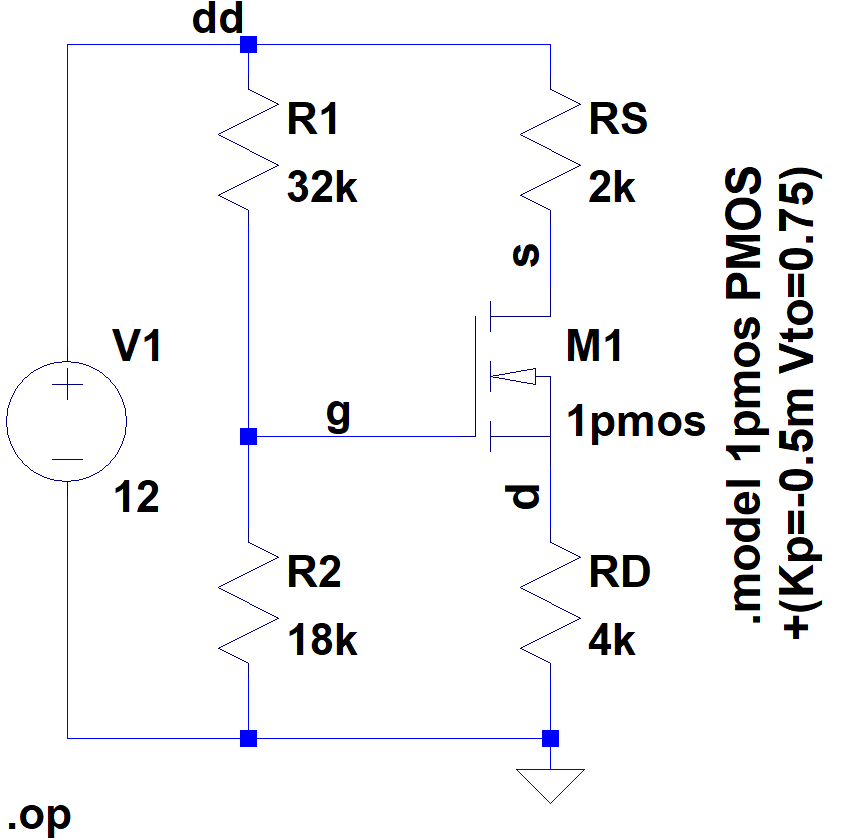
\includegraphics[width=.47\textwidth, height=\textheight, keepaspectratio=true]{ds2b}
%\end{paracol}
%\end{center}

This assignment should demonstrate a basic understanding of designing basic MOSFET circuits by adapting the widths and lengths of the transistors.

\textit{I have neither given nor received unauthorized assistance on this assignment.}


\end{raggedright}
\end{document}
